\chapter{Résultats et réponses à nos questions de recherche}

Nous avons ici un artefact de recherche qui initie la conception d'un outil entièrement automatisé, capable de couvrir plusieurs architectures et plusieurs compilateurs. Cet outil, présenté tout au long de ces chapitre précédents, permet d'obtenir des rapports précis sur la sécurité d'une bibliothèque cryptographique. 

\section{Motivation de la méthode expérimentale}

Notre objectif est d'automatiser le processus de vérification d'un binaire d'une fonction d'une bibliothèque cryptographique. Nous savons effectuer ce travail localement, avec un fichier à tester, une compilation effectué avec plusieurs compilateurs et une analyse Binsec adapté à chaque version (\eg figures \ref{tab:resultats_arm} et \ref{tab:resultats_riscv}). Ce mécanisme, permettant une comparaison nette et forte entre les compilateurs est analogue à la méthode du parcours en largeur. Nous testons une variété de compilateur et les résultats obtenues au fur et à mesure nous permette d'évaluer une fonction à chaque fois.\medbreak

La méthode développé intrésèquement avec Érysichthon est analogue au parcours en profondeur. Nous étudions toute la bibliothèque (ou du moins les fonctions présentent dans la liste des cibles autorisés) selon les paramètres ciblés avant de considérer réaliser une analyse vers une autre configuration (architecture / compilateur / optimisation). Cette approche demande une réflexion concernant le choix de la configuration puis sera plus tard ajouté à une liste de configuration à analyser. Les rapports obtenues permettent d'identifier plus rapidement quelles fonctions ont besoin d'être corrigés mais surtout de repérer les éventuels bogues qui peuvent survenir.\smallbreak

Cette méthode nous a permis d'obtenir nos premier rapports. Nous allons maintenant discuter des résultats récoltés.

\section{Étude simple sur x86\_64}

L'exécution s'est réalisé sur une machine équipée d'un processeur \textit{Intel Xeon E5-2620v4} avec 32 Gio de mémoire. Le temps nécessaire pour une analyse complète en x86\_64 avec \texttt{GCC 12.02} avec les options de compilations courante est de 4h07 en moyenne. Une analyse complète comprend la compilation de HACL*, la génération des fichiers de tests, la compilation desdits fichiers et l'analyse individuelle de chacun par Binsec. La génération des rapports se fait en fin d'analyse de Binsec avant qu'une nouvelle compilation de HACL* ne soit réaliser. Le rapport consiste à aggréger les rapports d'analyse Binsec, compter les évènements que l'on cible et dresser des tableaux.\medbreak

La configuration de notre première étude est donc : [x86\_64, \texttt{GCC 12.02}, \texttt{-O}0/1/2/3/s/z].\medbreak

\begin{figure}[!ht]
  \centering
  \scalebox{0.65}{%
    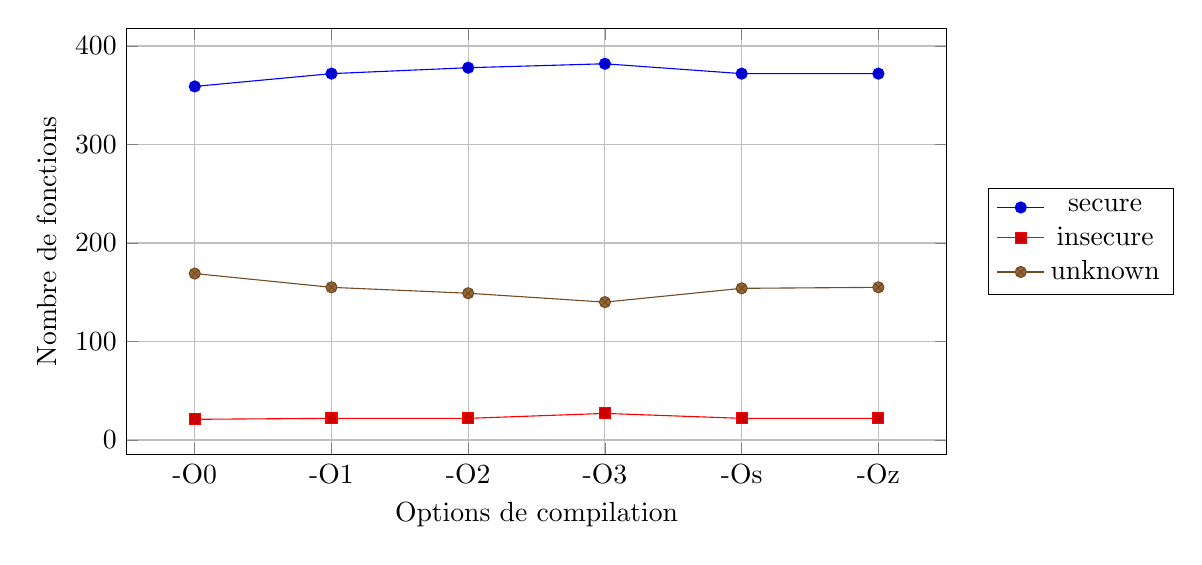
\begin{tikzpicture}
      \begin{axis}[
        xlabel={Options de compilation},
        ylabel={Nombre de fonctions},
        legend style={at={(0.5,-0.15)},anchor=north,legend columns=-1},
        grid=both,
        xtick={0,1,2,3,4,5},
        xticklabels={-O0, -O1, -O2, -O3, -Os, -Oz},
        width=12cm, height=7cm,
        legend style={at={(1.05,0.5)}, anchor=west},
        legend columns=1
      ]

        \addplot coordinates {(0,359) (1,372) (2,378) (3,382) (4,372) (5,372)};
        \addlegendentry{secure}

        \addplot coordinates {(0,21) (1,22) (2,22) (3,27) (4,22) (5,22)};
        \addlegendentry{insecure}

        \addplot coordinates {(0,169) (1,155) (2,149) (3,140) (4,154) (5,155)};
        \addlegendentry{unknown}

      \end{axis}
    \end{tikzpicture}%
  }
  \caption{Graphes des résultats d'Érysichthon en x86\_64}
  \label{fig:graphe_total}
\end{figure}


Les données détaillées peuvent être consultées en annexe \ref{tab:resultats_finaux}. En l'état, l'analyse rapporte entre 139 et 168 fichiers (en fonction des options de compilations, voir la figure \ref{fig:graphe_total}) dont l'analyse n'a pu se terminer. Il faudrait observer plus en détails ces fichiers pour connaître les causes précises de ces arrêts. Nous pouvons faire dans un premier temps une analyse haut niveau des raisons probables de ces interruptions. \medbreak

\begin{figure}[!ht]
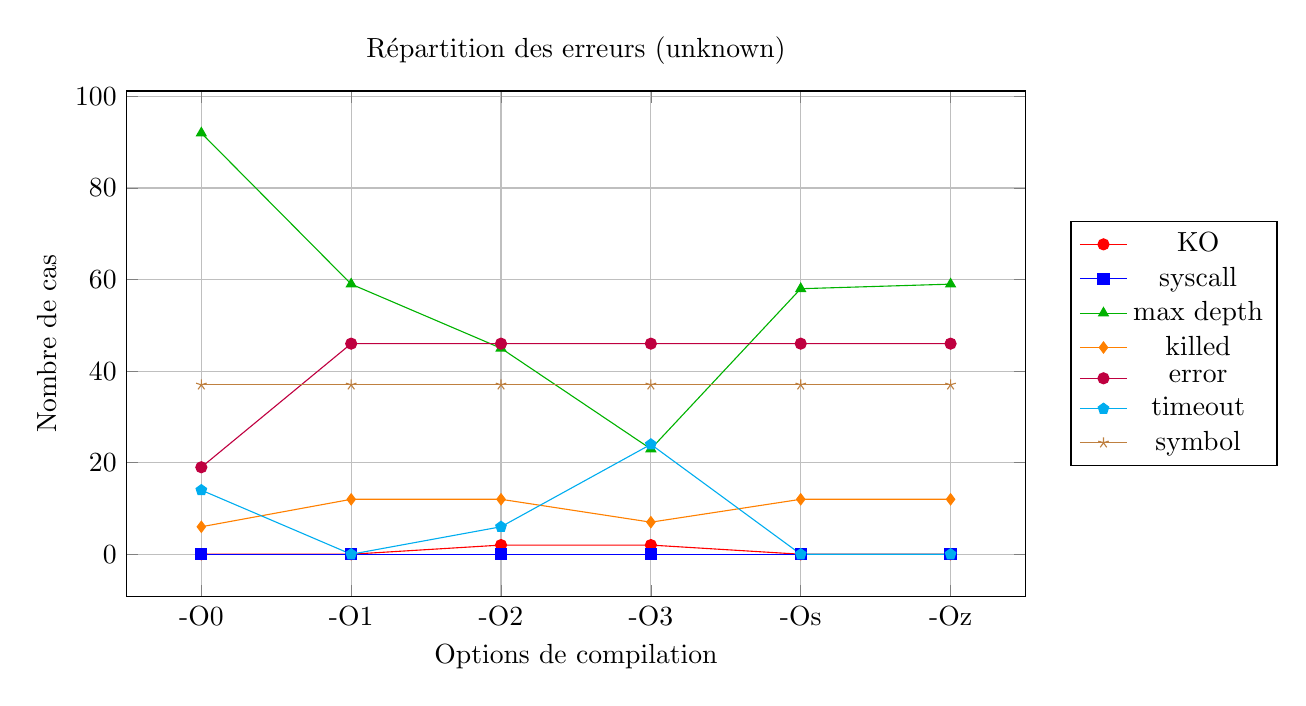
\begin{tikzpicture}
  \begin{axis}[
    title={Répartition des erreurs (unknown)},
    xlabel={Options de compilation},
    ylabel={Nombre de cas},
    grid=both,
    xtick={0,1,2,3,4,5},
    xticklabels={-O0, -O1, -O2, -O3, -Os, -Oz},
    width=13cm, height=8cm,
    legend style={at={(1.05,0.5)}, anchor=west}
  ]

    % KO
    \addplot[color=red, mark=*] coordinates {(0,0) (1,0) (2,2) (3,2) (4,0) (5,0)};
    \addlegendentry{KO}

    % syscall
    \addplot[color=blue, mark=square*] coordinates {(0,0) (1,0) (2,0) (3,0) (4,0) (5,0)};
    \addlegendentry{syscall}

    % max depth
    \addplot[color=green!70!black, mark=triangle*] coordinates {(0,92) (1,59) (2,45) (3,23) (4,58) (5,59)};
    \addlegendentry{max depth}

    % killed
    \addplot[color=orange, mark=diamond*] coordinates {(0,6) (1,12) (2,12) (3,7) (4,12) (5,12)};
    \addlegendentry{killed}

    % error
    \addplot[color=purple, mark=otimes*] coordinates {(0,19) (1,46) (2,46) (3,46) (4,46) (5,46)};
    \addlegendentry{error}

    % timeout
    \addplot[color=cyan, mark=pentagon*] coordinates {(0,14) (1,0) (2,6) (3,24) (4,0) (5,0)};
    \addlegendentry{timeout}

    % symbol
    \addplot[color=brown, mark=star] coordinates {(0,37) (1,37) (2,37) (3,37) (4,37) (5,37)};
    \addlegendentry{symbol}

  \end{axis}
\end{tikzpicture}
  \caption{Graphes détaillant les erreurs interrompant l'analyse Binsec}
  \label{fig:graphe_unknown}
\end{figure}

Le détail des valeurs est rapporté en annexe \ref{table:detail_unknown}.\smallbreak

On peut voir avec cette figure \ref{fig:graphe_unknown} que les erreurs sont dues à :
\begin{enumerate}
  \item[\texttt{max depth}] Arrêt par limitations du nombre d'instruction à analyser, cela permet de réduire la profondeur des branchement conditionnels à explorer et limiter le risque de parcours infini.
  \item[\texttt{timeout}] Comme le précédent, limitation par le temps. 
  \item[\texttt{killed}] Consommation excessive des ressources, processus interrompu. 
  \item[\texttt{error}] Instruction inconnue de Binsec, il a besoin que le script d'instruction soit corrigé.
  \item[\texttt{symbol}] Comme le précédent, mais peut-être que le fichier de test a besoin d'être modifié.
  \item[\texttt{KO}] Instruction inconnue de Binsec, il a besoin d'être amélioré. 
\end{enumerate}

Chaque erreur préconise un correctif à apporter à Érysichthon. Nous allons détailler les solutions qui nous sont apparus.

\subsection*{Correctifs à implémenter}

Pour résoudre la limitation \texttt{max depth}, nous utiliserons l'outil \texttt{perf}. Cela nous permet de déterminer le nombre d'instructions que contient le binaire. Identifier cette variable nous permet d'exécuter la commande \ref{lst:commande_binsec} précisément.\smallbreak

Concernant l'erreur de type \texttt{timeout}, par défaut une exécution Binsec ne s'interrompt pas, nous avions ajouter ce garde-fou pour forcé l'arrêt de l'analyse de certaines fonctions qui s'étendaient dans le temps. Nos scripts Binsec peuvent être affiné en ciblant précisément les fonctions qui ont besoin de cette limitation. Actuellement, il est sûrement préférable de retirer cette option.\smallbreak

Cela nous amène à l'erreur \texttt{killed}. Ce message n'est pas une erreur provoqué par Binsec mais par un moniteur externe qui vérifie que l'exécution d'Érysichthon ne consomme pas toute la mémoire vive de la machine hôte. Comme présenté au chapitre \ref{chap:erysichtonConception}, l'analyse d'un fichier binaire évolue exponentiellement. Il se trouve que ces fonctions sont comme un sandwich de plus petites fonctions et font exploser la complexité des formules SMT. L'erreur \texttt{max depth} n'est pas déclenché donc il faut sûrement affiné le script Binsec pour ces fonctions.

L'erreur \texttt{symbol} indique une erreur présente dans le scrit Binsec. Cela signifie que le fichier binaire n'a pas le symbole observé par Binsec. Cette erreur est dû à un fichier de test produit par Andhrímnir où deux fonctions utilisent des paramètres nommés identiquements. Cette erreur se corrige donc en améliorant le module Andhrímnir.

Pour finir, \texttt{KO} et \texttt{error} sont des erreurs provoqués par Binsec. Dans le premier cas l'instruction binaire lui ait inconnu et dans le second cas il effectue une analyse vers un segment du binaire qu'il n'arrive pas à lire, il faut donc modifier le script pour éviter ce cas de figures.


\subsection*{Sécurité de HACL*}

Revenons sur les resultats présentés sur la figure \ref{fig:graphe_total} et ignorons les fonctions marquées \texttt{unknown}. Les fichiers non sécurisés sont les plus nombreux avec l'option \texttt{-O3} (27) et le moins avec l'option \texttt{-O0} (21). Nous retrouvons le détail des résultats en annexe \ref{tab:resultats_insecure}. Cette expérimentation confirme les travaux de \citeauthor{schneider2024breakingbadcompilersbreak}, dans le sens où augmenter le niveau d'optimisation de compilation augmente le nombre de fonctions qui sont non sécurisés. Nos résultats pourront s'aligner avec l'ajout du compilateur \texttt{LLVM}.\smallbreak 

En revanche, si la question de la sécurité des fonctions identifiées non sécurisées se posent, actuellement la réponse est non. Comme nous analysons toute la bibliothèque HACL*, il est normal que certaines fonctions ne soient pas sécurisées. Elle n'ont pas pour objectif de l'être. Ce sont des fonctions comme \texttt{Hacl\_P256\_\-vali\-date\_public\_key} ou \texttt{Hacl\_P256\_\-ecdsa\_\-verif\_p256\_sha384} qui effectuent des vérifications, des conversions, sur des données publiques. 

Actuellement, dans la liste, aucune fonction indiquée non sécurisé ne demande une réimplémentation et peut être conservé dans la bibliothèque. En première conclusion préliminaire, nous pouvons affirmer qu'il est préférable de ne pas utiliser l'option de compilation \texttt{-O3}.


